% Options for packages loaded elsewhere
\PassOptionsToPackage{unicode}{hyperref}
\PassOptionsToPackage{hyphens}{url}
%
\documentclass[
  letterpaper,
  oneside,
  open=any]{scrbook}

\usepackage{amsmath,amssymb}
\usepackage{iftex}
\ifPDFTeX
  \usepackage[T1]{fontenc}
  \usepackage[utf8]{inputenc}
  \usepackage{textcomp} % provide euro and other symbols
\else % if luatex or xetex
  \usepackage{unicode-math}
  \defaultfontfeatures{Scale=MatchLowercase}
  \defaultfontfeatures[\rmfamily]{Ligatures=TeX,Scale=1}
\fi
\usepackage{lmodern}
\ifPDFTeX\else  
    % xetex/luatex font selection
\fi
% Use upquote if available, for straight quotes in verbatim environments
\IfFileExists{upquote.sty}{\usepackage{upquote}}{}
\IfFileExists{microtype.sty}{% use microtype if available
  \usepackage[]{microtype}
  \UseMicrotypeSet[protrusion]{basicmath} % disable protrusion for tt fonts
}{}
\makeatletter
\@ifundefined{KOMAClassName}{% if non-KOMA class
  \IfFileExists{parskip.sty}{%
    \usepackage{parskip}
  }{% else
    \setlength{\parindent}{0pt}
    \setlength{\parskip}{6pt plus 2pt minus 1pt}}
}{% if KOMA class
  \KOMAoptions{parskip=half}}
\makeatother
\usepackage{xcolor}
\setlength{\emergencystretch}{3em} % prevent overfull lines
\setcounter{secnumdepth}{5}
% Make \paragraph and \subparagraph free-standing
\makeatletter
\ifx\paragraph\undefined\else
  \let\oldparagraph\paragraph
  \renewcommand{\paragraph}{
    \@ifstar
      \xxxParagraphStar
      \xxxParagraphNoStar
  }
  \newcommand{\xxxParagraphStar}[1]{\oldparagraph*{#1}\mbox{}}
  \newcommand{\xxxParagraphNoStar}[1]{\oldparagraph{#1}\mbox{}}
\fi
\ifx\subparagraph\undefined\else
  \let\oldsubparagraph\subparagraph
  \renewcommand{\subparagraph}{
    \@ifstar
      \xxxSubParagraphStar
      \xxxSubParagraphNoStar
  }
  \newcommand{\xxxSubParagraphStar}[1]{\oldsubparagraph*{#1}\mbox{}}
  \newcommand{\xxxSubParagraphNoStar}[1]{\oldsubparagraph{#1}\mbox{}}
\fi
\makeatother
\usepackage{color}
\usepackage{fancyvrb}
\newcommand{\VerbBar}{|}
\newcommand{\VERB}{\Verb[commandchars=\\\{\}]}
\DefineVerbatimEnvironment{Highlighting}{Verbatim}{commandchars=\\\{\}}
% Add ',fontsize=\small' for more characters per line
\usepackage{framed}
\definecolor{shadecolor}{RGB}{241,243,245}
\newenvironment{Shaded}{\begin{snugshade}}{\end{snugshade}}
\newcommand{\AlertTok}[1]{\textcolor[rgb]{0.68,0.00,0.00}{#1}}
\newcommand{\AnnotationTok}[1]{\textcolor[rgb]{0.37,0.37,0.37}{#1}}
\newcommand{\AttributeTok}[1]{\textcolor[rgb]{0.40,0.45,0.13}{#1}}
\newcommand{\BaseNTok}[1]{\textcolor[rgb]{0.68,0.00,0.00}{#1}}
\newcommand{\BuiltInTok}[1]{\textcolor[rgb]{0.00,0.23,0.31}{#1}}
\newcommand{\CharTok}[1]{\textcolor[rgb]{0.13,0.47,0.30}{#1}}
\newcommand{\CommentTok}[1]{\textcolor[rgb]{0.37,0.37,0.37}{#1}}
\newcommand{\CommentVarTok}[1]{\textcolor[rgb]{0.37,0.37,0.37}{\textit{#1}}}
\newcommand{\ConstantTok}[1]{\textcolor[rgb]{0.56,0.35,0.01}{#1}}
\newcommand{\ControlFlowTok}[1]{\textcolor[rgb]{0.00,0.23,0.31}{\textbf{#1}}}
\newcommand{\DataTypeTok}[1]{\textcolor[rgb]{0.68,0.00,0.00}{#1}}
\newcommand{\DecValTok}[1]{\textcolor[rgb]{0.68,0.00,0.00}{#1}}
\newcommand{\DocumentationTok}[1]{\textcolor[rgb]{0.37,0.37,0.37}{\textit{#1}}}
\newcommand{\ErrorTok}[1]{\textcolor[rgb]{0.68,0.00,0.00}{#1}}
\newcommand{\ExtensionTok}[1]{\textcolor[rgb]{0.00,0.23,0.31}{#1}}
\newcommand{\FloatTok}[1]{\textcolor[rgb]{0.68,0.00,0.00}{#1}}
\newcommand{\FunctionTok}[1]{\textcolor[rgb]{0.28,0.35,0.67}{#1}}
\newcommand{\ImportTok}[1]{\textcolor[rgb]{0.00,0.46,0.62}{#1}}
\newcommand{\InformationTok}[1]{\textcolor[rgb]{0.37,0.37,0.37}{#1}}
\newcommand{\KeywordTok}[1]{\textcolor[rgb]{0.00,0.23,0.31}{\textbf{#1}}}
\newcommand{\NormalTok}[1]{\textcolor[rgb]{0.00,0.23,0.31}{#1}}
\newcommand{\OperatorTok}[1]{\textcolor[rgb]{0.37,0.37,0.37}{#1}}
\newcommand{\OtherTok}[1]{\textcolor[rgb]{0.00,0.23,0.31}{#1}}
\newcommand{\PreprocessorTok}[1]{\textcolor[rgb]{0.68,0.00,0.00}{#1}}
\newcommand{\RegionMarkerTok}[1]{\textcolor[rgb]{0.00,0.23,0.31}{#1}}
\newcommand{\SpecialCharTok}[1]{\textcolor[rgb]{0.37,0.37,0.37}{#1}}
\newcommand{\SpecialStringTok}[1]{\textcolor[rgb]{0.13,0.47,0.30}{#1}}
\newcommand{\StringTok}[1]{\textcolor[rgb]{0.13,0.47,0.30}{#1}}
\newcommand{\VariableTok}[1]{\textcolor[rgb]{0.07,0.07,0.07}{#1}}
\newcommand{\VerbatimStringTok}[1]{\textcolor[rgb]{0.13,0.47,0.30}{#1}}
\newcommand{\WarningTok}[1]{\textcolor[rgb]{0.37,0.37,0.37}{\textit{#1}}}

\providecommand{\tightlist}{%
  \setlength{\itemsep}{0pt}\setlength{\parskip}{0pt}}\usepackage{longtable,booktabs,array}
\usepackage{calc} % for calculating minipage widths
% Correct order of tables after \paragraph or \subparagraph
\usepackage{etoolbox}
\makeatletter
\patchcmd\longtable{\par}{\if@noskipsec\mbox{}\fi\par}{}{}
\makeatother
% Allow footnotes in longtable head/foot
\IfFileExists{footnotehyper.sty}{\usepackage{footnotehyper}}{\usepackage{footnote}}
\makesavenoteenv{longtable}
\usepackage{graphicx}
\makeatletter
\newsavebox\pandoc@box
\newcommand*\pandocbounded[1]{% scales image to fit in text height/width
  \sbox\pandoc@box{#1}%
  \Gscale@div\@tempa{\textheight}{\dimexpr\ht\pandoc@box+\dp\pandoc@box\relax}%
  \Gscale@div\@tempb{\linewidth}{\wd\pandoc@box}%
  \ifdim\@tempb\p@<\@tempa\p@\let\@tempa\@tempb\fi% select the smaller of both
  \ifdim\@tempa\p@<\p@\scalebox{\@tempa}{\usebox\pandoc@box}%
  \else\usebox{\pandoc@box}%
  \fi%
}
% Set default figure placement to htbp
\def\fps@figure{htbp}
\makeatother
% definitions for citeproc citations
\NewDocumentCommand\citeproctext{}{}
\NewDocumentCommand\citeproc{mm}{%
  \begingroup\def\citeproctext{#2}\cite{#1}\endgroup}
\makeatletter
 % allow citations to break across lines
 \let\@cite@ofmt\@firstofone
 % avoid brackets around text for \cite:
 \def\@biblabel#1{}
 \def\@cite#1#2{{#1\if@tempswa , #2\fi}}
\makeatother
\newlength{\cslhangindent}
\setlength{\cslhangindent}{1.5em}
\newlength{\csllabelwidth}
\setlength{\csllabelwidth}{3em}
\newenvironment{CSLReferences}[2] % #1 hanging-indent, #2 entry-spacing
 {\begin{list}{}{%
  \setlength{\itemindent}{0pt}
  \setlength{\leftmargin}{0pt}
  \setlength{\parsep}{0pt}
  % turn on hanging indent if param 1 is 1
  \ifodd #1
   \setlength{\leftmargin}{\cslhangindent}
   \setlength{\itemindent}{-1\cslhangindent}
  \fi
  % set entry spacing
  \setlength{\itemsep}{#2\baselineskip}}}
 {\end{list}}
\usepackage{calc}
\newcommand{\CSLBlock}[1]{\hfill\break\parbox[t]{\linewidth}{\strut\ignorespaces#1\strut}}
\newcommand{\CSLLeftMargin}[1]{\parbox[t]{\csllabelwidth}{\strut#1\strut}}
\newcommand{\CSLRightInline}[1]{\parbox[t]{\linewidth - \csllabelwidth}{\strut#1\strut}}
\newcommand{\CSLIndent}[1]{\hspace{\cslhangindent}#1}

\usepackage[default]{opensans}
\fontseries{lc}\selectfont
\makeatletter
\@ifpackageloaded{bookmark}{}{\usepackage{bookmark}}
\makeatother
\makeatletter
\@ifpackageloaded{caption}{}{\usepackage{caption}}
\AtBeginDocument{%
\ifdefined\contentsname
  \renewcommand*\contentsname{Table of contents}
\else
  \newcommand\contentsname{Table of contents}
\fi
\ifdefined\listfigurename
  \renewcommand*\listfigurename{List of Figures}
\else
  \newcommand\listfigurename{List of Figures}
\fi
\ifdefined\listtablename
  \renewcommand*\listtablename{List of Tables}
\else
  \newcommand\listtablename{List of Tables}
\fi
\ifdefined\figurename
  \renewcommand*\figurename{圖}
\else
  \newcommand\figurename{圖}
\fi
\ifdefined\tablename
  \renewcommand*\tablename{表}
\else
  \newcommand\tablename{表}
\fi
}
\@ifpackageloaded{float}{}{\usepackage{float}}
\floatstyle{ruled}
\@ifundefined{c@chapter}{\newfloat{codelisting}{h}{lop}}{\newfloat{codelisting}{h}{lop}[chapter]}
\floatname{codelisting}{Listing}
\newcommand*\listoflistings{\listof{codelisting}{List of Listings}}
\makeatother
\makeatletter
\makeatother
\makeatletter
\@ifpackageloaded{caption}{}{\usepackage{caption}}
\@ifpackageloaded{subcaption}{}{\usepackage{subcaption}}
\makeatother

\usepackage{hyphenat}
\usepackage{ifthen}
\usepackage{calc}
\usepackage{calculator}

\usepackage{graphicx}
\usepackage{wallpaper}

\usepackage{geometry}

\usepackage{graphicx}
\usepackage{geometry}
\usepackage{afterpage}
\usepackage{tikz}
\usetikzlibrary{calc}
\usetikzlibrary{fadings}
\usepackage[pagecolor=none]{pagecolor}


% Set the titlepage font families







% Set the coverpage font families


\usepackage{bookmark}

\IfFileExists{xurl.sty}{\usepackage{xurl}}{} % add URL line breaks if available
\urlstyle{same} % disable monospaced font for URLs
\hypersetup{
  pdftitle={白鯨記摘譯},
  hidelinks,
  pdfcreator={LaTeX via pandoc}}


\title{白鯨記摘譯}
\author{}
\date{}

\begin{document}
%%%%% begin titlepage extension code

  \begin{frontmatter}

\begin{titlepage}
% This is a combination of Pandoc templating and LaTeX
% Pandoc templating https://pandoc.org/MANUAL.html#templates
% See the README for help

\thispagestyle{empty}

\newgeometry{top=-100in}

% Page color

\newcommand{\coverauthorstyle}[1]{{\fontsize{20}{24.0}\selectfont
#1}}

\begin{tikzpicture}[remember picture, overlay, inner sep=0pt, outer sep=0pt]

\tikzfading[name=fadeout, inner color=transparent!0,outer color=transparent!100]
\tikzfading[name=fadein, inner color=transparent!100,outer color=transparent!0]
\node[anchor=south west, rotate=0.0, opacity=1.0] at ($(current page.south west)+(0pt, 8.75in)$) {

\includegraphics[width=\paperwidth, keepaspectratio]{images/cover-header-2.png}};

% Title
\newcommand{\titlelocationleft}{2.3in}
\newcommand{\titlelocationbottom}{7in}
\newcommand{\titlealign}{left}

\begin{scope}{%
\fontsize{30}{36.0}\selectfont
\node[anchor=north
west, align=left, rotate=0] (Title1) at ($(current page.south west)+(\titlelocationleft,\titlelocationbottom)$)  [text width = 5in]  {\textcolor{black}{\bfseries{\nohyphens{白鯨記摘譯}}}};
}
\end{scope}

% Header
\newcommand{\headerlocationleft}{2.3in}
\newcommand{\headerlocationbottom}{9.8in}
\newcommand{\headerlocationalign}{left}

\begin{scope}
{%
\fontsize{16}{19.2}\selectfont
 \node[anchor=north west, align=left, rotate=0] (Header1) at %
($(current page.south west)+(\headerlocationleft,\headerlocationbottom)$)  [text width = 5in]  {\textcolor{white}{\nohyphens{NOAA
Technical Memorandum NMFS-XXX-\#\#}}};
}
\end{scope}

% Footer
\newcommand{\footerlocationleft}{6in}
\newcommand{\footerlocationbottom}{0.1\paperheight}
\newcommand{\footerlocationalign}{left}

\begin{scope}
{%
\fontsize{8}{9.6}\selectfont
 \node[anchor=north west, align=left, rotate=0] (Footer1) at %
($(current page.south west)+(\footerlocationleft,\footerlocationbottom)$)  [text width = 2.5in]  {{\nohyphens{U.S.
DEPARTMENT OF COMMERCE\\
\strut \\
National Oceanic and Atmospheric Administration\\
National Marine Fisheries Service\\
Northwest Fisheries Science Center}}};
}
\end{scope}

% Date
\newcommand{\datelocationleft}{6in}
\newcommand{\datelocationbottom}{2in}
\newcommand{\datelocationalign}{left}

\begin{scope}
{%
\fontsize{20}{24.0}\selectfont
 \node[anchor=north west, align=left, rotate=0] (Date1) at %
($(current page.south west)+(\datelocationleft,\datelocationbottom)$)  [text width = 2.5in]  {{\nohyphens{January
2023}}};
}
\end{scope}

\end{tikzpicture}
\clearpage
\restoregeometry
%%% TITLE PAGE START

% Set up alignment commands
%Page
\newcommand{\titlepagepagealign}{
\ifthenelse{\equal{left}{right}}{\raggedleft}{}
\ifthenelse{\equal{left}{center}}{\centering}{}
\ifthenelse{\equal{left}{left}}{\raggedright}{}
}
%% Titles
\newcommand{\titlepagetitlealign}{
\ifthenelse{\equal{left}{right}}{\raggedleft}{}
\ifthenelse{\equal{left}{center}}{\centering}{}
\ifthenelse{\equal{left}{left}}{\raggedright}{}
\ifthenelse{\equal{left}{spread}}{\makebox[\linewidth][s]}{}
}


\newcommand{\titleandsubtitle}{
% Title and subtitle
{\fontsize{30}{36.0}\selectfont
\textcolor{black}{\bfseries{\nohyphens{白鯨記摘譯}}}\par
}%
}
\newcommand{\titlepagetitleblock}{
\titleandsubtitle
}

\newcommand{\authorstyle}[1]{{\fontsize{20}{24.0}\selectfont
#1}}

\newcommand{\affiliationstyle}[1]{{#1}}

\newcommand{\titlepageauthorblock}{
{\authorstyle{}}}

\newcommand{\titlepageaffiliationblock}{
\hangindent=1em
\hangafter=1
{\affiliationstyle{


\vspace{1\baselineskip} 
}}
}
\newcommand{\headerstyled}{%
{}
}
\newcommand{\footerstyled}{%
{}
}
\newcommand{\datestyled}{%
{}
}


\newcommand{\titlepageheaderblock}{\headerstyled}

\newcommand{\titlepagefooterblock}{
\footerstyled
}

\newcommand{\titlepagedateblock}{
\datestyled
}

%set up blocks so user can specify order
\newcommand{\titleblock}{{\titlepagetitlealign

{\titlepagetitleblock}
}

\vspace{4\baselineskip}
}

\newcommand{\authorblock}{}

\newcommand{\affiliationblock}{}

\newcommand{\logoblock}{}

\newcommand{\footerblock}{}

\newcommand{\dateblock}{}

\newcommand{\headerblock}{}
\newgeometry{top=3in,bottom=1in,right=1in,left=1.75in}
% background image
\newlength{\bgimagesize}
\setlength{\bgimagesize}{0.75\paperwidth}
\LENGTHDIVIDE{\bgimagesize}{\paperwidth}{\theRatio} % from calculator pkg
\ThisULCornerWallPaper{\theRatio}{images/corner-image.png}

\thispagestyle{empty} % no page numbers on titlepages


\newcommand{\vrulecode}{\rule{\vrulewidth}{\textheight}}
\newlength{\vrulewidth}
\setlength{\vrulewidth}{0pt}
\newlength{\B}
\setlength{\B}{\ifdim\vrulewidth > 0pt 0.05\textwidth\else 0pt\fi}
\newlength{\minipagewidth}
\ifthenelse{\equal{left}{left} \OR \equal{left}{right} }
{% True case
\setlength{\minipagewidth}{\textwidth - \vrulewidth - \B - 0.1\textwidth}
}{
\setlength{\minipagewidth}{\textwidth - 2\vrulewidth - 2\B - 0.1\textwidth}
}
\ifthenelse{\equal{left}{left} \OR \equal{left}{leftright}}
{% True case
\raggedleft % needed for the minipage to work
\vrulecode
\hspace{\B}
}{%
\raggedright % else it is right only and width is not 0
}
% [position of box][box height][inner position]{width}
% [s] means stretch out vertically; assuming there is a vfill
\begin{minipage}[b][\textheight][s]{\minipagewidth}
\titlepagepagealign
\headerblock

\titleblock

\authorblock

\affiliationblock

\vfill

\logoblock

\footerblock
\par

\end{minipage}\ifthenelse{\equal{left}{right} \OR \equal{left}{leftright} }{
\hspace{\B}
\vrulecode}{}
\clearpage
\restoregeometry
%%% TITLE PAGE END
\end{titlepage}
\setcounter{page}{1}
\end{frontmatter}

%%%%% end titlepage extension code

\renewcommand*\contentsname{Table of contents}
{
\setcounter{tocdepth}{1}
\tableofcontents
}
\listoffigures
\listoftables

\mainmatter
\bookmarksetup{startatroot}

\chapter*{Summary}\label{summary}
\addcontentsline{toc}{chapter}{Summary}

\markboth{Summary}{Summary}

白鯨記Lorem ipsum dolor sit amet, consectetur adipiscing elit. Integer
commodo gravida justo consectetur condimentum. Proin eget felis non nunc
tristique malesuada vel ut tortor. Vivamus lacinia aliquet lorem in
congue. In hac habitasse platea dictumst. Etiam non felis iaculis,
efficitur libero in, porta nunc. Sed sit amet nisi non justo scelerisque
feugiat. Pellentesque porta consectetur sapien, porttitor iaculis ligula
fermentum ac. Pellentesque fermentum elementum lacus non tempus. Aenean
eu leo lobortis, vulputate mi at, varius sapien. In congue consectetur
ultricies. Maecenas volutpat facilisis arcu, eget sodales tellus
consequat nec. Integer ullamcorper ex nec leo aliquam tempus. Orci
varius natoque penatibus et magnis dis parturient montes, nascetur
ridiculus mus. Nunc dui massa, facilisis at aliquet eu, malesuada vel
neque. Donec fermentum elit eu tortor euismod, sed mollis lacus blandit.

\bookmarksetup{startatroot}

\chapter{第一章}\label{ux7b2cux4e00ux7ae0}

\section{軟體分類}\label{ux8edfux9ad4ux5206ux985e}

在網際網路出現以前,尤其是大型主機(mainframe)的年代,傳統上將軟體大抵分為系統軟體(system
software)及應用軟體(application
software)二大類。系統軟體通常指由電腦硬體製造商所開發,用來搭配硬體運行的軟體,例如,作業系統或週邊設備的驅動程式;系統軟體通常是由電腦製造商在設備出廠時即附隨發行,後續可能視需要發行新版本。
應用軟體則是部署在系統軟體上執行,用來協助處理業務的軟體,例如,銀行的存款資訊系統、企業的財務管理資訊系統等。這類應用軟體多是由企業內部的IT部門,或是委由軟體公司,根據企業的需求開發軟體。

隨著個人電腦及網際網路普及,另一種分類是從軟體服務的對象及其功能性質著眼,將軟體分成通用型軟體(generic
software)及定製型軟體(customed
software)二大類。通用型軟體是為普遍使用所設計的軟體,可以滿足許多客戶的一般要求,通常是以現成產品(commercial
off-the-shielf,
COTS)的方式發行,公開在市場上販售。此類產品的例子包括用於各種行動裝置的應用程式(APP)、用於
PC
的軟體(文字處理器-Word、電子試算表及繪圖軟體等),廣義來說,也包括為特定領域所設計的垂直應用系統(vertical
applications),例如圖書館資訊系統、會計系統,或醫療診所的掛號及病歷管理系統等。
客製型軟體則是根據客戶預先定義的規格,委託軟體開發公司(或由組織內部的IT部門自行發展),為滿足客戶的特定需求而開發的軟體,只提供給特定的客戶或使用者操作使用。此類軟體通常是為支援特定的業務流程,例如,道路交通管制系統、空氣品質監測資料管理系統、公務機關的入口網站等。

通用型軟體和定製型軟體的關鍵區別在於,通用性軟體的規格是由開發者所掌握及控制,這意味著,如果他們遇到開發或是後續維護上的問題,他們可以重新調整或更新其內容。對於客製性軟體,其需求及規格則由委託的客戶所製定及規範,承攬開發的軟體公司必須按照客戶所要求的規格開發軟體。詳如
圖~\ref{fig-sw-category} 的說明

\begin{figure}

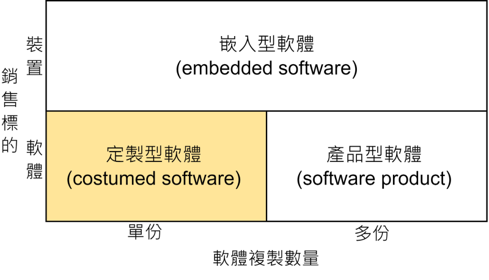
\includegraphics[width=3.125in,height=\textheight,keepaspectratio]{content/../images/sw-category.png}

\caption{\label{fig-sw-category}軟體的分類}

\end{figure}%

\begin{center}\rule{0.5\linewidth}{0.5pt}\end{center}

\section{軟體需求的定義}\label{ux8edfux9ad4ux9700ux6c42ux7684ux5b9aux7fa9}

軟體需求(Software
Requirements)是指在開發軟體系統時,對系統功能、性能、行為、設計約束及其他相關特性的描述。這些需求是軟體開發過程中的基礎,用於指導設計、開發、測試和維護工作。

\begin{center}\rule{0.5\linewidth}{0.5pt}\end{center}

\section{IEEE
對軟體需求的定義}\label{ieee-ux5c0dux8edfux9ad4ux9700ux6c42ux7684ux5b9aux7fa9}

根據 \textbf{IEEE 610.12-1990} 標準,軟體需求被定義為:

\begin{enumerate}
\def\labelenumi{\arabic{enumi}.}
\item
  \textbf{使用者需求(User Requirements)}:\\
  從使用者角度描述系統應提供的功能與特性,通常以自然語言或圖表形式表達,便於非技術人員理解。
\item
  \textbf{系統需求(System Requirements)}:\\
  詳細描述系統應實現的功能、性能、設計約束及其他特性,通常以技術性語言表達,供開發團隊使用。
\item
  \textbf{軟體需求規格(Software Requirements Specification, SRS)}:\\
  這是一份正式文件,詳細記錄軟體系統的所有需求,包括功能需求、非功能需求及設計約束。
\end{enumerate}

\begin{center}\rule{0.5\linewidth}{0.5pt}\end{center}

\bookmarksetup{startatroot}

\chapter{Customize}\label{customize}

\section{Edit and add your pages}\label{edit-and-add-your-pages}

Edit the qmd or md files in the \texttt{content} folder. qmd files can
include code (R, Python, Julia) and lots of Quarto markdown bells and
whistles (like call-outs, cross-references, auto-citations and much
more).

Each page should start with

\begin{verbatim}
---
title: your title
---
\end{verbatim}

and the first header will be the 2nd level, so \texttt{\#\#}. Note,
there are situations where you leave off

\begin{verbatim}
---
title: your title
---
\end{verbatim}

and start the qmd file with a level header \texttt{\#}, but if using the
default title yaml (in the \texttt{-\/-\/-} fence) is a good habit since
it makes it easy for Quarto convert your qmd file to other formats (like
into a presentation).

\section{Add your pages the project}\label{add-your-pages-the-project}

\begin{itemize}
\tightlist
\item
  Add the files to \texttt{\_quarto.yml}
\end{itemize}

\bookmarksetup{startatroot}

\chapter{Customization}\label{customization}

\section{Quarto documentation}\label{quarto-documentation}

Quarto allow many bells and whistles to make nice output. Read the
documentation here \href{https://quarto.org/docs/guide/}{Quarto
documentation}.

\section{Examples}\label{examples}

Looking at other people's Quarto code is a great way to figure out how
to do stuff. Most will have a link to a GitHub repo where you can see
the raw code. Look for a link to edit page or see source code. This will
usually be on the right. Or look for the GitHub icon somewhere.

\begin{itemize}
\tightlist
\item
  \href{https://quarto.org/docs/gallery/}{Quarto gallery}
\item
  \href{https://nmfs-openscapes.github.io/}{nmfs-openscapes}
\item
  \href{https://thefaylab.github.io/lab-manual/}{Faye lab manual}
\item
  \href{https://nmfs-opensci.github.io/quarto_titlepages/}{quarto-titlepages}
  Note the link to edit is broken. Go to repo and look in
  \texttt{documentation} directory.
\end{itemize}

\bookmarksetup{startatroot}

\chapter{Rendering}\label{rendering}

The repo includes a GitHub Action that will render (build) the website
automatically when you make changes to the files. It will be pushed to
the \texttt{gh-pages} branch.

But when you are developing your content, you will want to render it
locally.

\section{Step 1. Make sure you have a recent
RStudio}\label{step-1.-make-sure-you-have-a-recent-rstudio}

Have you updated RStudio since about August 2022? No? Then update to a
newer version of RStudio. In general, you want to keep RStudio updated
and it is required to have a recent version to use Quarto.

\section{Step 2. Clone and create RStudio
project}\label{step-2.-clone-and-create-rstudio-project}

First, clone the repo onto your local computer. How? You can click File
\textgreater{} New Project and then select ``Version Control''. Paste in
the url of the repository. That will clone the repo on to your local
computer. When you make changes, you will need to push those up.

\section{Step 3. Render within
RStudio}\label{step-3.-render-within-rstudio}

RStudio will recognize that this is a Quarto project by the presence of
the \texttt{\_quarto.yml} file and will see the ``Build'' tab. Click the
``Render website'' button to render to the \texttt{\_site} folder.

\textbf{Previewing:} You can either click \texttt{index.html} in the
\texttt{\_site} folder and specify ``preview in browser'' or set up
RStudio to preview to the viewer panel. To do the latter, go to Tools
\textgreater{} Global Options \textgreater{} R Markdown. Then select
``Show output preview in: Viewer panel''.

\bookmarksetup{startatroot}

\chapter{Figures and Tables}\label{figures-and-tables}

Markdown is a simple formatting syntax for authoring HTML, PDF, and MS
Word documents. For more details on using R Markdown see
\url{http://rmarkdown.rstudio.com}.

\section{Code}\label{code}

You can embed an R code chunk like this:

\begin{Shaded}
\begin{Highlighting}[]
\FunctionTok{summary}\NormalTok{(cars)}
\end{Highlighting}
\end{Shaded}

\begin{verbatim}
     speed           dist       
 Min.   : 4.0   Min.   :  2.00  
 1st Qu.:12.0   1st Qu.: 26.00  
 Median :15.0   Median : 36.00  
 Mean   :15.4   Mean   : 42.98  
 3rd Qu.:19.0   3rd Qu.: 56.00  
 Max.   :25.0   Max.   :120.00  
\end{verbatim}

\section{Including Plots}\label{including-plots}

You can also embed plots and reference them, like so
圖~\ref{fig-pressure}.

\begin{figure}

\centering{

\pandocbounded{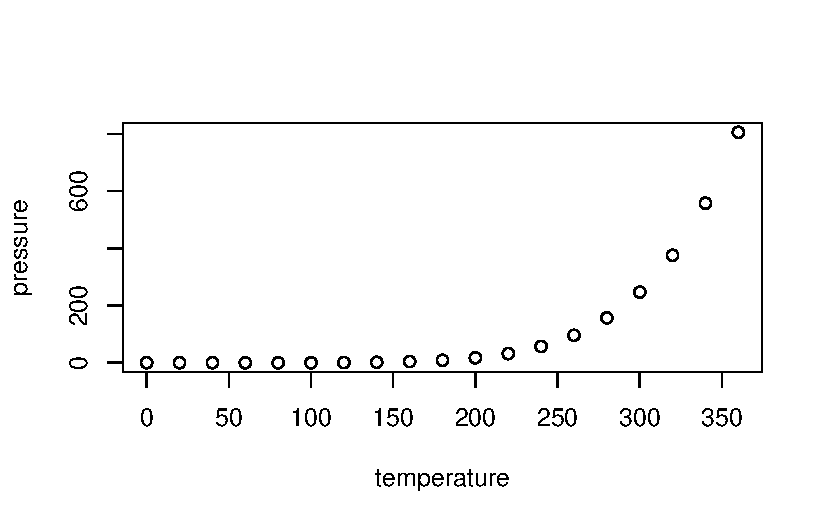
\includegraphics[keepaspectratio]{content/figures_and_tables_files/figure-pdf/fig-pressure-1.pdf}}

}

\caption{\label{fig-pressure}Plot of pressure}

\end{figure}%

Note that the \texttt{echo\ =\ FALSE} parameter was added to the code
chunk to prevent printing of the R code that generated the plot.

\section{Including Tables}\label{including-tables}

You can also embed tables and reference them with 表~\ref{tbl-iris}.

\begin{Shaded}
\begin{Highlighting}[]
\FunctionTok{library}\NormalTok{(knitr)}
\FunctionTok{kable}\NormalTok{(}\FunctionTok{head}\NormalTok{(iris))}
\end{Highlighting}
\end{Shaded}

\begin{longtable}[]{@{}rrrrl@{}}

\caption{\label{tbl-iris}Iris Data}

\tabularnewline

\toprule\noalign{}
Sepal.Length & Sepal.Width & Petal.Length & Petal.Width & Species \\
\midrule\noalign{}
\endhead
\bottomrule\noalign{}
\endlastfoot
5.1 & 3.5 & 1.4 & 0.2 & setosa \\
4.9 & 3.0 & 1.4 & 0.2 & setosa \\
4.7 & 3.2 & 1.3 & 0.2 & setosa \\
4.6 & 3.1 & 1.5 & 0.2 & setosa \\
5.0 & 3.6 & 1.4 & 0.2 & setosa \\
5.4 & 3.9 & 1.7 & 0.4 & setosa \\

\end{longtable}

\bookmarksetup{startatroot}

\chapter{Rendering with Code}\label{rendering-with-code}

You can have code (R, Python or Julia) in your qmd file. You will need
to have these installed on your local computer, but presumably you do
already if you are adding code to your qmd files.

\begin{Shaded}
\begin{Highlighting}[]
\NormalTok{x }\OtherTok{\textless{}{-}} \FunctionTok{c}\NormalTok{(}\DecValTok{5}\NormalTok{, }\DecValTok{15}\NormalTok{, }\DecValTok{25}\NormalTok{, }\DecValTok{35}\NormalTok{, }\DecValTok{45}\NormalTok{, }\DecValTok{55}\NormalTok{)}
\NormalTok{y }\OtherTok{\textless{}{-}} \FunctionTok{c}\NormalTok{(}\DecValTok{5}\NormalTok{, }\DecValTok{20}\NormalTok{, }\DecValTok{14}\NormalTok{, }\DecValTok{32}\NormalTok{, }\DecValTok{22}\NormalTok{, }\DecValTok{38}\NormalTok{)}
\FunctionTok{lm}\NormalTok{(x }\SpecialCharTok{\textasciitilde{}}\NormalTok{ y)}
\end{Highlighting}
\end{Shaded}

\begin{verbatim}

Call:
lm(formula = x ~ y)

Coefficients:
(Intercept)            y  
      1.056        1.326  
\end{verbatim}

\section{Modify the GitHub Action}\label{modify-the-github-action}

You will need to change the GitHub Action in \texttt{.github/workflows}
to install these and any needed packages in order for GitHub to be able
to render your webpage. The GitHub Action install R since I used that in
\texttt{code.qmd}. If you use Python or Julia instead, then you will
need to update the GitHub Action to install those.

If getting the GitHub Action to work is too much hassle (and that
definitely happens), you can alway render locally and publish to the
\texttt{gh-pages} branch. If you do this, make sure to delete or rename
the GitHub Action to something like

\begin{verbatim}
render-and-publish.old_yml
\end{verbatim}

so GitHub does not keep trying to run it. Nothing bad will happen if you
don't do this, but if you are not using the action (because it keeps
failing), then you don't need GitHub to run it.

\section{Render locally and publish to gh-pages
branch}\label{render-locally-and-publish-to-gh-pages-branch}

To render locally and push up to the \texttt{gh-pages} branch, open a
terminal window and then \texttt{cd} to the directory with the Quarto
project. Type this in the terminal:

\begin{verbatim}
quarto render gh-pages
\end{verbatim}

\bookmarksetup{startatroot}

\chapter{References}\label{references}

Quarto has powerful references functionality. You can easily insert
citations from Zotero libraries that you maintain in the cloud (on
Zotero). This allows the whole team to update the library and you can
sync up to that library. Read about this on the Quarto documentation on
\href{https://quarto.org/docs/visual-editor/technical.html\#citations}{citations}.
Google youtube videos on this also to see it in action.

Add a \texttt{.bib} file in to your project or add a linked Zotero
library via RStudio in Visual mode with Tools \textgreater{} Project
Options\ldots{} \textgreater{} R Markdown \textgreater{} select custom
libraries from the Zotero dropdown.

The you can type \texttt{@} and you will see a dropdown of the
references in your libraries. You can then select the ones to add. If
you don't see the one you need, you can paste in the DOI and it will be
added to your references file (with all the info). The references will
be added to your references section of your book automatically.

See the \texttt{references.qmd} file for how to include the references.

\begin{itemize}
\item
  \texttt{@ansley1981} will produce Ansley and Davis (1981)
\item
  \texttt{{[}@ansley1981{]}} will produce (Ansley and Davis 1981).
\end{itemize}

\bookmarksetup{startatroot}

\chapter*{References}\label{references-1}
\addcontentsline{toc}{chapter}{References}

\markboth{References}{References}

\phantomsection\label{refs}
\begin{CSLReferences}{1}{0}
\bibitem[\citeproctext]{ref-ansley1981}
Ansley, H. L. H., and C. D. Davis. 1981. {``Migration and Standing Stock
of Fishes Associated with Artificial and Natural Reefs on Georgia{'}s
Outer Continental Shelf.''} Brunswick, Georgia, USA.

\end{CSLReferences}


\backmatter


\end{document}
